% ============================================================================
% Discrete Mathematics - Practical 2-3 (Relations): pedagogical solutions.
% English, pdflatex. Source is ASCII-clean: no em-dash, no en-dash, no straight quote glyphs.
% Compile: pdflatex twice.
% ============================================================================
\documentclass[11pt,a4paper]{article}

% ---- Encoding & fonts ----
\usepackage[utf8]{inputenc}
\usepackage[T1]{fontenc}
\usepackage{lmodern}

% ---- Math ----
\usepackage{amsmath,amssymb,amsthm}
\usepackage{mathtools}

% ---- Layout ----
\usepackage[margin=2.3cm]{geometry}
\usepackage{enumitem}
\usepackage{booktabs}
\usepackage{array}

% ---- Visuals ----
\usepackage{xcolor}
\usepackage[most]{tcolorbox}
\usepackage{tikz}
\usetikzlibrary{arrows.meta,positioning,calc,fit,backgrounds,shapes.misc,decorations.pathreplacing}
\usepackage{pgfplots}
\pgfplotsset{compat=1.18}
\usepackage{hyperref}
\hypersetup{colorlinks=true,linkcolor=blue!55!black,urlcolor=blue!55!black}

% ---- Palette (Armenian flag colours; use for 3+ series plots) ----
\definecolor{armRed}{HTML}{D90012}
\definecolor{armBlue}{HTML}{0033A0}
\definecolor{armOrange}{HTML}{F2A800}
\definecolor{ink}{HTML}{22303C}

\setlength{\parindent}{0pt}
\setlength{\parskip}{5pt}

% ---- Math shortcuts ----
\newcommand{\Z}{\mathbb{Z}}
\newcommand{\R}{\mathbb{R}}
\newcommand{\N}{\mathbb{N}}
\newcommand{\Q}{\mathbb{Q}}
\DeclareMathOperator{\Dom}{D}
\DeclareMathOperator{\Ran}{R}

% ---- Boxes ----
\newtcolorbox{problembox}[1][]{enhanced, breakable, sharp corners=south,
  colback=armOrange!10, colframe=armOrange!75!black, boxrule=0.8pt, arc=2mm,
  fonttitle=\bfseries\color{white}, coltitle=white,
  attach boxed title to top left={xshift=4mm,yshift=-2.4mm},
  boxed title style={colback=armOrange!85!black, arc=1mm},
  title={Problem #1}}

\newtcolorbox{ideabox}{enhanced, breakable,
  colback=armBlue!6, colframe=armBlue!70!black, boxrule=0.8pt, arc=2mm,
  fonttitle=\bfseries\color{white}, coltitle=white,
  attach boxed title to top left={xshift=4mm,yshift=-2.4mm},
  boxed title style={colback=armBlue!75!black, arc=1mm},
  title={The idea}}

\newtcolorbox{methodbox}{enhanced, breakable,
  colback=gray!8, colframe=gray!55!black, boxrule=0.7pt, arc=2mm,
  fonttitle=\bfseries, title={$\bigstar$\ Method to remember}}

\newtcolorbox{answerbox}{enhanced, sharp corners=south,
  colback=green!8, colframe=green!50!black, boxrule=1pt, arc=2mm, left=4mm,right=4mm}
\newcommand{\answer}[1]{\begin{answerbox}\centering\textbf{Answer:}\quad #1\end{answerbox}}

% ---- Title ----
\title{\vspace{-1.2cm}\textbf{Discrete Mathematics - Practical 2-3}\\[2pt]
\large Relations: worked solutions\\[2pt]
\normalsize\itshape with the reasoning spelled out, step by step}
\author{}
\date{}

\begin{document}
\maketitle
\vspace{-1.0cm}

\section*{Warm-up: what a relation is, and why we draw it}

A (binary) relation $\rho$ on sets is just a \emph{set of ordered pairs}. Writing
$(x,y)\in\rho$ (also $x\,\rho\,y$) means \textquotedbl{}$x$ is related to $y$\textquotedbl{}.
That is the whole definition - but a bare list of pairs hides everything interesting, so a relation
is almost always better understood as a \textbf{picture}:

\begin{itemize}[leftmargin=1.4em,itemsep=2pt,topsep=2pt]
\item On a finite set, draw a \textbf{graph}: a dot for each element and an arrow $x\to y$ for each
  pair $(x,y)\in\rho$. If the relation is symmetric we drop the arrowheads and draw plain edges.
\item The same data is a 0/1 \textbf{adjacency matrix} $M$: put $M_{ij}=1$ exactly when
  (element $i$, element $j$) $\in\rho$. The graph and the matrix are two views of one object.
\item On $\R^2$ a relation is a \textbf{region or curve in the plane}; its domain and range are the
  shadows it casts on the $x$- and $y$-axes.
\end{itemize}

We use the course's conventions throughout. The \textbf{domain} is the set of first coordinates,
$\Dom_\rho=\{x:\exists y\,(x,y)\in\rho\}$, and the \textbf{range} is the set of second coordinates,
$\Ran_\rho=\{y:\exists x\,(x,y)\in\rho\}$. \textbf{Composition is left-to-right}: $\rho\cdot\sigma$
means \textquotedbl{}do $\rho$ first, then $\sigma$\textquotedbl{}, i.e.
$(x,z)\in\rho\cdot\sigma \iff \exists y:\ (x,y)\in\rho\ \text{and}\ (y,z)\in\sigma$. (This is the
opposite order to the $\circ$ many books use, so watch the direction.) Here $\N=\{1,2,3,\dots\}$.

% ============================================================================
\section*{Problem 1.2 - Domain and range}
% ============================================================================

\begin{problembox}[1.2]
Find the domain $\Dom_\rho$ and range $\Ran_\rho$ of each relation.
\\[2pt]
\begin{tabular}{@{}ll@{}}
a) $\{(a,1),(a,2),(c,1),(c,2),(c,4),(d,5)\}$ &
e) $\{(x,y)\in\N^2 : y\mid x\}$\ \ (source: $x/y$)\\
b) $\{(1,2),(2,4),(3,6),(4,8),\dots\}=\{(n,2n)\}$ &
f) $\{(x,y)\in\N^2 : x\mid y\}$\ \ (source: $y/x$)\\
c) $\{(x,y)\in\R^2 : x=y^2\}$ &
g) $\{(x,y)\in\R^2 : x+y\le 0\}$\\
d) $\{(x,y)\in\R^2 : x^2+y^2\le 16\}$ &
h) $\{(x,y)\in\R^2 : 2x\ge 3y\}$
\end{tabular}
\\[3pt]
\footnotesize Here the sheet's notation $x/y$ is the divisibility predicate
\textquotedbl{}$x$ over $y$ is a whole number\textquotedbl{}, i.e. $y\mid x$ in (e), and $x\mid y$ in (f).
\end{problembox}

\begin{ideabox}
Domain and range are \textbf{shadows}. Stand a light to the side and let the relation cast its
shadow on the $x$-axis: that shadow is the domain (which $x$-values appear as a first coordinate).
Shine from below onto the $y$-axis and the shadow is the range. So you never need the whole relation
at once - you only ask, for each candidate $x$, \textbf{\textquotedbl{}is there at least one $y$
that partners it?\textquotedbl{}} If yes, $x$ is in the domain. Same question with the roles of
$x$ and $y$ swapped gives the range. For the plane relations, draw the region and read the two
shadows off the axes; for the discrete ones, a single witnessing partner settles each value.
\end{ideabox}

\textbf{(a) Finite list - just read it off.}
First coordinates: $a,c,d$. Second coordinates: $1,2,4,5$.
\[\Dom=\{a,c,d\},\qquad \Ran=\{1,2,4,5\}.\]

\textbf{(b) The doubling relation $\{(n,2n)\}$.}
Every $n\in\N$ is a first coordinate, so $\Dom=\N$. The second coordinates are exactly the even
numbers, so $\Ran=\{2,4,6,\dots\}=2\N$.

\textbf{(c), (d), (g), (h) - the plane relations.} Draw each, then read the shadows.

\begin{center}
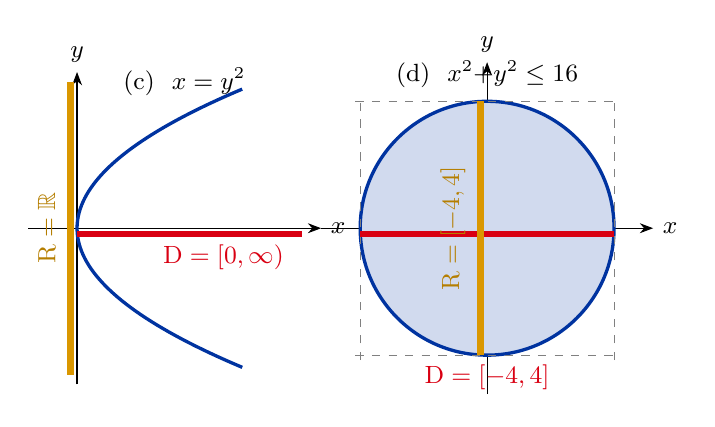
\begin{tikzpicture}[scale=0.62, font=\small, >=Stealth]
% ---------- (c) x = y^2 : sideways parabola ----------
\begin{scope}
  \draw[->] (-1,0)--(5,0) node[right]{$x$};
  \draw[->] (0,-3.2)--(0,3.2) node[above]{$y$};
  \draw[armBlue,very thick,domain=-2.85:2.85,samples=80,variable=\t]
        plot ({\t*\t/2.4},{\t});  % x scaled so curve fits; shape is x=y^2
  % domain shadow on x-axis: [0,inf)
  \draw[armRed,line width=2.4pt] (0,-0.12)--(4.6,-0.12);
  \node[armRed] at (3.0,-0.6) {$\Dom=[0,\infty)$};
  % range shadow on y-axis: all R
  \draw[armOrange!90!black,line width=2.4pt] (-0.13,-3)--(-0.13,3);
  \node[armOrange!75!black,rotate=90] at (-0.62,0) {$\Ran=\R$};
  \node at (2.2,3.0) {(c)\ \ $x=y^2$};
\end{scope}
% ---------- (d) disk x^2+y^2<=16 ----------
\begin{scope}[xshift=8.4cm]
  \draw[->] (-3.4,0)--(3.4,0) node[right]{$x$};
  \draw[->] (0,-3.4)--(0,3.4) node[above]{$y$};
  \fill[armBlue!18] (0,0) circle (2.6);
  \draw[armBlue,very thick] (0,0) circle (2.6);
  \foreach \v in {-2.6,2.6}{
     \draw[dashed,gray] (\v,-2.7)--(\v,2.7);
     \draw[dashed,gray] (-2.7,\v)--(2.7,\v);}
  \draw[armRed,line width=2.4pt] (-2.6,-0.12)--(2.6,-0.12);
  \node[armRed] at (0,-3.05) {$\Dom=[-4,4]$};
  \draw[armOrange!90!black,line width=2.4pt] (-0.13,-2.6)--(-0.13,2.6);
  \node[armOrange!75!black,rotate=90] at (-0.7,0) {$\Ran=[-4,4]$};
  \node at (0,3.15) {(d)\ \ $x^2{+}y^2\le 16$};
\end{scope}
\end{tikzpicture}
\end{center}

\begin{center}
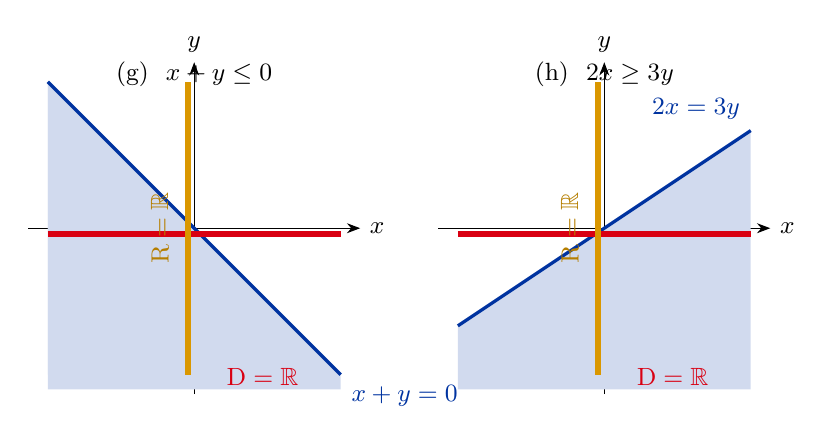
\begin{tikzpicture}[scale=0.62, font=\small, >=Stealth]
% ---------- (g) x+y<=0 : half-plane below line y=-x ----------
\begin{scope}
  \draw[->] (-3.4,0)--(3.4,0) node[right]{$x$};
  \draw[->] (0,-3.4)--(0,3.4) node[above]{$y$};
  \fill[armBlue!16] (-3,3)--(-3,-3)--(3,-3)--(3,-3)-- (-3,3)--cycle; % placeholder
  % half-plane y <= -x : below the line through (-3,3),(3,-3)
  \fill[armBlue!18] (-3,3)--(3,-3)--(3,-3.3)--(-3,-3.3)--cycle;
  \draw[armBlue,very thick] (-3,3)--(3,-3) node[below right]{$x+y=0$};
  \draw[armRed,line width=2.0pt] (-3,-0.12)--(3,-0.12);
  \node[armRed] at (1.4,-3.05) {$\Dom=\R$};
  \draw[armOrange!90!black,line width=2.0pt] (-0.13,-3)--(-0.13,3);
  \node[armOrange!75!black,rotate=90] at (-0.7,0) {$\Ran=\R$};
  \node at (0,3.15) {(g)\ \ $x+y\le 0$};
\end{scope}
% ---------- (h) 2x>=3y : half-plane y<=2x/3 ----------
\begin{scope}[xshift=8.4cm]
  \draw[->] (-3.4,0)--(3.4,0) node[right]{$x$};
  \draw[->] (0,-3.4)--(0,3.4) node[above]{$y$};
  % line y = 2x/3 : through (-3,-2),(3,2). region y <= 2x/3 is below it.
  \fill[armBlue!18] (-3,-2)--(3,2)--(3,-3.3)--(-3,-3.3)--cycle;
  \draw[armBlue,very thick] (-3,-2)--(3,2) node[above left]{$2x=3y$};
  \draw[armRed,line width=2.0pt] (-3,-0.12)--(3,-0.12);
  \node[armRed] at (1.4,-3.05) {$\Dom=\R$};
  \draw[armOrange!90!black,line width=2.0pt] (-0.13,-3)--(-0.13,3);
  \node[armOrange!75!black,rotate=90] at (-0.7,0) {$\Ran=\R$};
  \node at (0,3.15) {(h)\ \ $2x\ge 3y$};
\end{scope}
\end{tikzpicture}
\end{center}

\textbf{(c) $x=y^2$.} The curve is a parabola opening along the positive $x$-axis. An $x$ appears
iff $x=y^2$ has a solution, i.e. iff $x\ge0$; so $\Dom=[0,\infty)$. Any real $y$ partners the point
$x=y^2$, so every $y$ appears: $\Ran=\R$.

\textbf{(d) the disk $x^2+y^2\le16$.} Radius $\sqrt{16}=4$. A value $x$ appears iff some $y$ has
$x^2+y^2\le16$; the easiest partner is $y=0$, which works iff $x^2\le16$, i.e. $x\in[-4,4]$.
By symmetry $\Ran=[-4,4]$ too.

\textbf{(g) $x+y\le0$.} The region is the closed half-plane on and below the line $x+y=0$. Given any
$x$, pick $y\le-x$ (e.g. $y=-x$); given any $y$, pick $x\le-y$. Every real works on both sides, so
$\Dom=\Ran=\R$.

\textbf{(h) $2x\ge3y$.} Half-plane on and below the line $2x=3y$ (that is $y=\tfrac23 x$). Given any
$x$, take $y\le\tfrac{2x}{3}$; given any $y$, take $x\ge\tfrac{3y}{2}$. Again $\Dom=\Ran=\R$.

\textbf{(e), (f) - divisibility on $\N$.} Recall $y\mid x$ means $y$ divides $x$.
For (e) ($y\mid x$): every $x\in\N$ is divisible by $y=1$, so $x$ always has a partner, $\Dom=\N$;
and every $y$ divides $x=y$ itself, so $y$ always appears, $\Ran=\N$. For (f) ($x\mid y$) the same
argument with $x,y$ swapped gives $\Dom=\N$ and $\Ran=\N$.

\textbf{Always check.} The Python enumeration over $1\le x,y\le199$ for (e),(f) produced every value
$1,\dots,199$ in both the domain and the range, and the bounded plane samples confirmed
$\Dom_c=[0,\infty)$, $\Dom_d=\Ran_d=[-4,4]$, and $\Dom=\Ran=\R$ for (g),(h). \checkmark

\begin{center}
\renewcommand{\arraystretch}{1.2}
\begin{tabular}{@{}c|cc@{}}
\toprule
 & $\Dom$ & $\Ran$\\
\midrule
a) & $\{a,c,d\}$ & $\{1,2,4,5\}$\\
b) & $\N$ & $2\N=\{2,4,6,\dots\}$\\
c) & $[0,\infty)$ & $\R$\\
d) & $[-4,4]$ & $[-4,4]$\\
e) & $\N$ & $\N$\\
f) & $\N$ & $\N$\\
g) & $\R$ & $\R$\\
h) & $\R$ & $\R$\\
\bottomrule
\end{tabular}
\end{center}

\answer{See the table above: domains and ranges for (a)--(h).}

\begin{methodbox}
\textbf{Transferable technique:} domain and range are the two axis-shadows of the relation. To test
if a value $x_0$ is in the domain you do not need the whole picture - just exhibit \emph{one}
partner $y$ with $(x_0,y)\in\rho$. For relations in $\R^2$, sketch the region and literally read the
shadows; for an equation $x=f(y)$ the domain is the set of outputs of $f$ and the range is $f$'s
input set.
\end{methodbox}

% ============================================================================
\section*{Problem 2.1 - Undirected graph and adjacency matrix}
% ============================================================================

\begin{problembox}[2.1]
On $A=\{a,b,c,d,e\}$ build the graph and the adjacency matrix of each relation (rows and columns
ordered $a,b,c,d,e$).
\begin{itemize}[leftmargin=1.6em,nosep]
\item[a)] $\{(a,b),(b,a),(b,c),(c,b),(c,a),(a,c),(d,e),(e,d)\}$
\item[b)] $\{(a,b),(b,a),(b,c),(c,b),(c,d),(d,c),(c,a),(a,c)\}$
\item[c)] same set as (b) in the source.
\end{itemize}
\end{problembox}

\begin{ideabox}
Each pair $(i,j)$ in the relation is one $1$ in the matrix (row $i$, column $j$) and one arrow
$i\to j$ in the graph. Here every relation is \textbf{symmetric}: whenever $(i,j)$ is present so is
$(j,i)$. Symmetry shows up two ways at once - in the matrix as $M=M^{\mathsf T}$ (it is mirror-image
across the diagonal), and in the graph as \textquotedbl{}every arrow has its reverse\textquotedbl{},
so we may erase the arrowheads and draw a single undirected \textbf{edge} per mutual pair. Reading
the picture is then just counting edges; reading the matrix is just checking the mirror.
\end{ideabox}

\textbf{Step 1 - List the undirected edges.}
(a) The mutual pairs give edges $a\!-\!b$, $b\!-\!c$, $a\!-\!c$ (a triangle on $a,b,c$) and a
separate edge $d\!-\!e$. (b) Edges $a\!-\!b$, $b\!-\!c$, $a\!-\!c$ (triangle again) plus $c\!-\!d$;
vertex $e$ has no edge. (c) is identical to (b).

\textbf{Step 2 - Draw and write the matrix side by side.}

\begin{center}
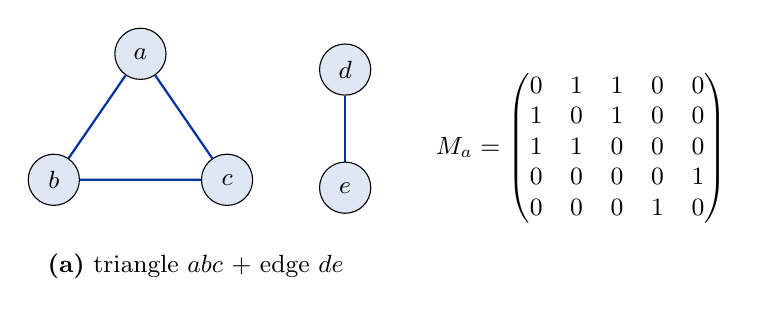
\begin{tikzpicture}[font=\small,
  vtx/.style={circle,draw,fill=armBlue!12,minimum size=6.5mm,inner sep=0pt}]
% --- (a) ---
\begin{scope}
  \node[vtx] (a) at (0,1.6) {$a$};
  \node[vtx] (b) at (-1.1,0) {$b$};
  \node[vtx] (c) at (1.1,0) {$c$};
  \node[vtx] (d) at (2.6,1.4) {$d$};
  \node[vtx] (e) at (2.6,-0.1) {$e$};
  \draw[armBlue,thick] (a)--(b)--(c)--(a);
  \draw[armBlue,thick] (d)--(e);
  \node at (0.7,-1.1) {\textbf{(a)} triangle $abc$ $+$ edge $de$};
\end{scope}
\node at (5.6,0.4) {$M_a=\begin{pmatrix}
0&1&1&0&0\\ 1&0&1&0&0\\ 1&1&0&0&0\\ 0&0&0&0&1\\ 0&0&0&1&0
\end{pmatrix}$};
\end{tikzpicture}
\end{center}

\begin{center}
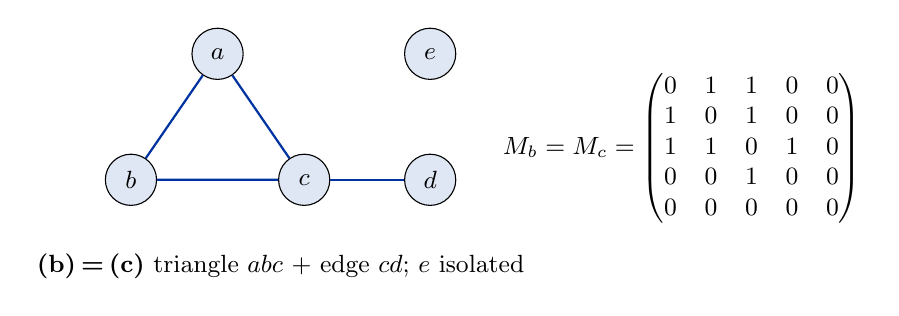
\begin{tikzpicture}[font=\small,
  vtx/.style={circle,draw,fill=armBlue!12,minimum size=6.5mm,inner sep=0pt}]
% --- (b)=(c) ---
\begin{scope}
  \node[vtx] (a) at (0,1.6) {$a$};
  \node[vtx] (b) at (-1.1,0) {$b$};
  \node[vtx] (c) at (1.1,0) {$c$};
  \node[vtx] (d) at (2.7,0) {$d$};
  \node[vtx] (e) at (2.7,1.6) {$e$};
  \draw[armBlue,thick] (a)--(b)--(c)--(a);
  \draw[armBlue,thick] (c)--(d);
  \node at (0.8,-1.1) {\textbf{(b)\,=\,(c)} triangle $abc$ $+$ edge $cd$; $e$ isolated};
\end{scope}
\node at (5.9,0.4) {$M_b=M_c=\begin{pmatrix}
0&1&1&0&0\\ 1&0&1&0&0\\ 1&1&0&1&0\\ 0&0&1&0&0\\ 0&0&0&0&0
\end{pmatrix}$};
\end{tikzpicture}
\end{center}

\textbf{Always check.} Each matrix is mirror-symmetric across the main diagonal (as it must be for a
symmetric relation), the diagonal is all $0$ (no pair $(x,x)$ is listed), and the number of $1$s
equals twice the number of edges: (a) $8$ ones $=2\times4$ edges, (b) $8$ ones $=2\times4$ edges.
The Python check confirmed both matrices entry-for-entry and that each is symmetric. \checkmark

\answer{(a) triangle $abc$ plus edge $de$; (b)=(c) triangle $abc$ plus edge $cd$, $e$ isolated. Matrices as drawn.}

\begin{methodbox}
\textbf{Transferable technique:} a symmetric relation $\Leftrightarrow$ an undirected graph
$\Leftrightarrow$ a symmetric 0/1 matrix. Count of $1$s $=2\cdot(\#\text{edges})$, and the diagonal
records the loops $(x,x)$. To sanity-check a hand-drawn graph against its matrix, verify $M=M^{\mathsf T}$.
\end{methodbox}

% ============================================================================
\section*{Problem 2.2 - Directed graph (digraph) and adjacency matrix}
% ============================================================================

\begin{problembox}[2.2]
On $A=\{a,b,c,d,e,f\}$ build the digraph and the adjacency matrix of each relation
(order $a,b,c,d,e,f$). An arrow goes $i\to j$ exactly when $(i,j)\in\rho$.
\begin{itemize}[leftmargin=1.6em,nosep]
\item[a)] $\{(a,b),(b,c),(a,c),(b,e),(c,f),(c,d),(d,f),(f,e)\}$
\item[b)] $\{(a,b),(b,c),(d,c),(d,e),(f,e),(f,a),(b,e)\}$
\item[c)] $\{(a,c),(c,c),(c,d),(c,e),(e,c),(e,e),(e,f),(a,e)\}$
\end{itemize}
\end{problembox}

\begin{ideabox}
A general relation need not be symmetric, so we keep the \textbf{arrowheads}: $(i,j)$ is an arrow
\emph{from} $i$ \emph{to} $j$, and it need not come with the reverse arrow $j\to i$. In the matrix
this means $M$ is no longer mirror-symmetric: row $i$ tells you where you can go \emph{from} $i$,
column $j$ tells you what points \emph{to} $j$. A pair $(x,x)$ is a \textbf{self-loop} at $x$ and a
$1$ on the diagonal. Drawing the digraph is the fastest way to see structure the list hides
(\textquotedbl{}is there a path from $a$ to $f$? a cycle?\textquotedbl{}).
\end{ideabox}

\textbf{Read the matrices off the lists} (row $=$ source, column $=$ target):

\begin{center}
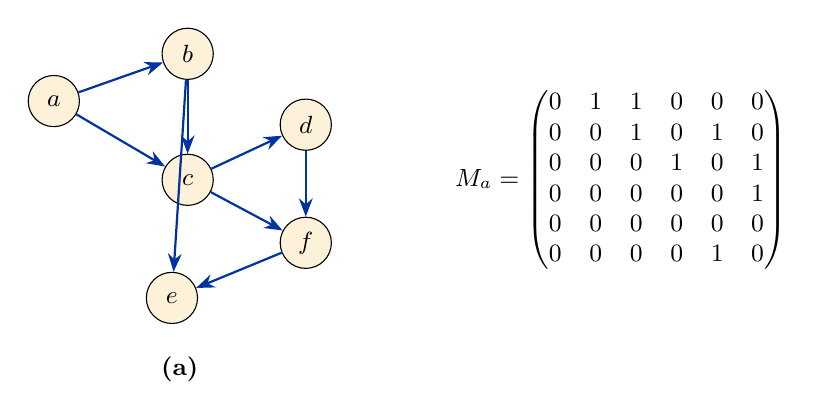
\begin{tikzpicture}[font=\small, >=Stealth,
  vtx/.style={circle,draw,fill=armOrange!15,minimum size=6.5mm,inner sep=0pt}]
% --- (a) digraph ---
  \node[vtx] (a) at (0,2) {$a$};
  \node[vtx] (b) at (1.7,2.6) {$b$};
  \node[vtx] (c) at (1.7,1.0) {$c$};
  \node[vtx] (d) at (3.2,1.7) {$d$};
  \node[vtx] (f) at (3.2,0.2) {$f$};
  \node[vtx] (e) at (1.5,-0.5) {$e$};
  \draw[armBlue,thick,->] (a)--(b);
  \draw[armBlue,thick,->] (a)--(c);
  \draw[armBlue,thick,->] (b)--(c);
  \draw[armBlue,thick,->] (b)--(e);
  \draw[armBlue,thick,->] (c)--(d);
  \draw[armBlue,thick,->] (c)--(f);
  \draw[armBlue,thick,->] (d)--(f);
  \draw[armBlue,thick,->] (f)--(e);
  \node at (1.6,-1.4) {\textbf{(a)}};
\node at (7.2,1.0) {$M_a=\begin{pmatrix}
0&1&1&0&0&0\\ 0&0&1&0&1&0\\ 0&0&0&1&0&1\\ 0&0&0&0&0&1\\ 0&0&0&0&0&0\\ 0&0&0&0&1&0
\end{pmatrix}$};
\end{tikzpicture}
\end{center}

\begin{center}
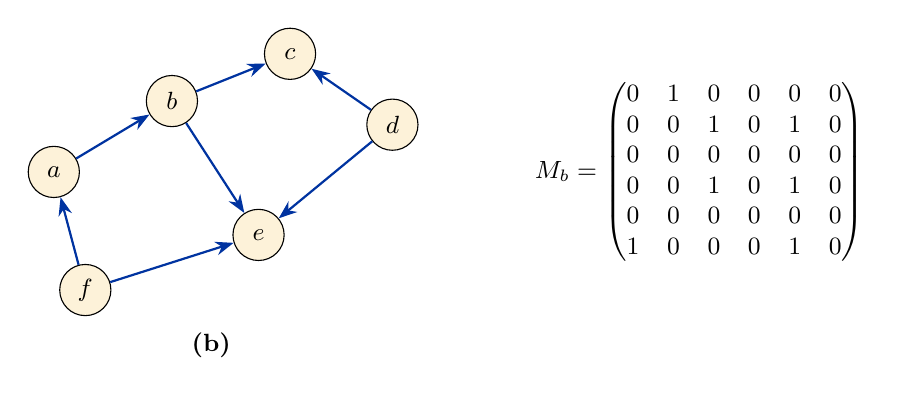
\begin{tikzpicture}[font=\small, >=Stealth,
  vtx/.style={circle,draw,fill=armOrange!15,minimum size=6.5mm,inner sep=0pt}]
% --- (b) digraph ---
  \node[vtx] (a) at (0,0) {$a$};
  \node[vtx] (b) at (1.5,0.9) {$b$};
  \node[vtx] (c) at (3.0,1.5) {$c$};
  \node[vtx] (d) at (4.3,0.6) {$d$};
  \node[vtx] (e) at (2.6,-0.8) {$e$};
  \node[vtx] (f) at (0.4,-1.5) {$f$};
  \draw[armBlue,thick,->] (a)--(b);
  \draw[armBlue,thick,->] (b)--(c);
  \draw[armBlue,thick,->] (b)--(e);
  \draw[armBlue,thick,->] (d)--(c);
  \draw[armBlue,thick,->] (d)--(e);
  \draw[armBlue,thick,->] (f)--(a);
  \draw[armBlue,thick,->] (f)--(e);
  \node at (2.0,-2.2) {\textbf{(b)}};
\node at (8.2,0) {$M_b=\begin{pmatrix}
0&1&0&0&0&0\\ 0&0&1&0&1&0\\ 0&0&0&0&0&0\\ 0&0&1&0&1&0\\ 0&0&0&0&0&0\\ 1&0&0&0&1&0
\end{pmatrix}$};
\end{tikzpicture}
\end{center}

\begin{center}
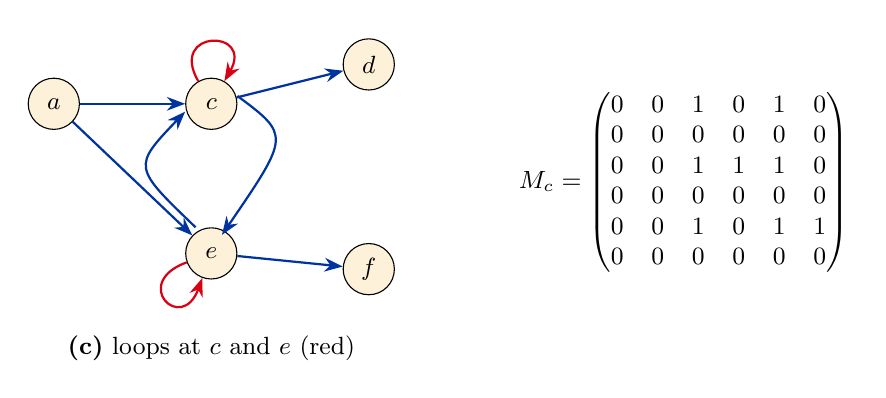
\begin{tikzpicture}[font=\small, >=Stealth,
  vtx/.style={circle,draw,fill=armOrange!15,minimum size=6.5mm,inner sep=0pt}]
% --- (c) digraph with loops ---
  \node[vtx] (a) at (0,1.4) {$a$};
  \node[vtx] (c) at (2.0,1.4) {$c$};
  \node[vtx] (e) at (2.0,-0.5) {$e$};
  \node[vtx] (d) at (4.0,1.9) {$d$};
  \node[vtx] (f) at (4.0,-0.7) {$f$};
  \draw[armBlue,thick,->] (a)--(c);
  \draw[armBlue,thick,->] (a)--(e);
  \draw[armBlue,thick,->] (c)--(d);
  \draw[armBlue,thick,->] ([yshift=1mm]c.east) .. controls (3.0,1.0) .. ([xshift=-1mm]e.north east);
  \draw[armBlue,thick,->] ([xshift=-2mm]e.north) .. controls (1.0,0.6) .. ([yshift=-1mm]c.west);
  \draw[armBlue,thick,->] (e)--(f);
  % loop at c
  \draw[armRed,thick,->] (c) .. controls +(120:1.1) and +(60:1.1) .. (c);
  % loop at e
  \draw[armRed,thick,->] (e) .. controls +(200:1.1) and +(250:1.1) .. (e);
  \node at (2.0,-1.7) {\textbf{(c)} loops at $c$ and $e$ (red)};
\node at (8.0,0.4) {$M_c=\begin{pmatrix}
0&0&1&0&1&0\\ 0&0&0&0&0&0\\ 0&0&1&1&1&0\\ 0&0&0&0&0&0\\ 0&0&1&0&1&1\\ 0&0&0&0&0&0
\end{pmatrix}$};
\end{tikzpicture}
\end{center}

\textbf{Always check.} Count the arrows in each list: (a) $8$, (b) $7$, (c) $8$; these equal the
number of $1$s in $M_a,M_b,M_c$ respectively. The two diagonal $1$s of $M_c$ are exactly the loops
$(c,c)$ and $(e,e)$ we drew in red. The Python check confirmed all three matrices entry-for-entry
and the loop positions. \checkmark

\answer{Digraphs as drawn; matrices $M_a,M_b,M_c$ as shown. Only (c) has self-loops, at $c$ and $e$.}

\begin{methodbox}
\textbf{Transferable technique:} for a general (directed) relation, $M_{ij}=1\iff i\to j$. Asymmetry
of the relation $=$ asymmetry of $M$; a self-loop $=$ a $1$ on the diagonal. \emph{Row $i$} lists the
out-neighbours of $i$; \emph{column $j$} lists the in-neighbours of $j$. A fast cross-check: number of
arrows $=$ number of $1$s.
\end{methodbox}

% ============================================================================
\section*{Problem 3.3 - Composition of two relations}
% ============================================================================

\begin{problembox}[3.3]
On $\Z$ let $\rho=\{(x,x+2):x\in\Z\}$ (the map $x\mapsto x+2$) and
$\sigma=\{(x,x^2):x\in\Z\}$ (the map $x\mapsto x^2$). Find $\rho\cdot\sigma$ and $\sigma\cdot\rho$.
\end{problembox}

\begin{ideabox}
Composition chains two relations through a \textbf{shared middle value}. With the course's
left-to-right rule, $\rho\cdot\sigma$ means \textquotedbl{}do $\rho$, then $\sigma$\textquotedbl{}:
start at $x$, let $\rho$ carry you to some $y$, then let $\sigma$ carry $y$ onward to $z$. The middle
$y$ is the hinge; the output relation pairs the original $x$ with the final $z$. Because both $\rho$
and $\sigma$ are \emph{functions} here (each input has exactly one output), the composition is just
\textbf{function composition} - and the order matters, because adding $2$ then squaring is not the
same as squaring then adding $2$.
\end{ideabox}

\textbf{Step 1 - $\rho\cdot\sigma$ (apply $\rho$ first).}
Start at $x$. $\rho$ sends $x\mapsto y=x+2$. Then $\sigma$ sends $y\mapsto z=y^2=(x+2)^2$. So
\[\rho\cdot\sigma=\{(x,(x+2)^2):x\in\Z\}.\]

\textbf{Step 2 - $\sigma\cdot\rho$ (apply $\sigma$ first).}
Start at $x$. $\sigma$ sends $x\mapsto y=x^2$. Then $\rho$ sends $y\mapsto z=y+2=x^2+2$. So
\[\sigma\cdot\rho=\{(x,x^2+2):x\in\Z\}.\]

\textbf{Step 3 - they are different.} $(x+2)^2=x^2+4x+4\neq x^2+2$ in general. A single value proves
it: at $x=1$, $\rho\cdot\sigma$ gives $(1,9)$ while $\sigma\cdot\rho$ gives $(1,3)$.

\textbf{The arrow diagram.} Tracking $x=1$ through the shared middle value makes the asymmetry visible:

\begin{center}
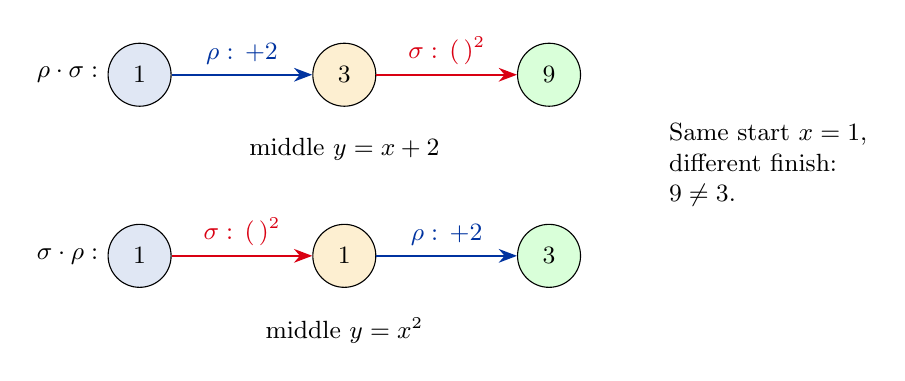
\begin{tikzpicture}[font=\small, >=Stealth, node distance=10mm,
  num/.style={circle,draw,minimum size=8mm,inner sep=0pt}]
% rho . sigma : 1 -(rho:+2)-> 3 -(sigma:^2)-> 9
\begin{scope}
  \node[num,fill=armBlue!12] (x1) at (0,0) {$1$};
  \node[num,fill=armOrange!18] (m1) at (2.6,0) {$3$};
  \node[num,fill=green!15] (z1) at (5.2,0) {$9$};
  \draw[armBlue,thick,->] (x1) -- node[above]{$\rho:\,+2$} (m1);
  \draw[armRed,thick,->] (m1) -- node[above]{$\sigma:\,(\,)^2$} (z1);
  \node[anchor=east] at (-0.4,0) {$\rho\cdot\sigma:$};
  \node at (2.6,-0.95) {middle $y=x+2$};
\end{scope}
% sigma . rho : 1 -(sigma:^2)-> 1 -(rho:+2)-> 3
\begin{scope}[yshift=-2.3cm]
  \node[num,fill=armBlue!12] (x2) at (0,0) {$1$};
  \node[num,fill=armOrange!18] (m2) at (2.6,0) {$1$};
  \node[num,fill=green!15] (z2) at (5.2,0) {$3$};
  \draw[armRed,thick,->] (x2) -- node[above]{$\sigma:\,(\,)^2$} (m2);
  \draw[armBlue,thick,->] (m2) -- node[above]{$\rho:\,+2$} (z2);
  \node[anchor=east] at (-0.4,0) {$\sigma\cdot\rho:$};
  \node at (2.6,-0.95) {middle $y=x^2$};
\end{scope}
\node[align=left,anchor=west] at (6.6,-1.15)
  {Same start $x=1$,\\ different finish:\\ $9\neq 3$.};
\end{tikzpicture}
\end{center}

\textbf{Always check.} The Python enumeration over $-20\le x\le 20$ gave $\rho\cdot\sigma$ output
$(x+2)^2$ and $\sigma\cdot\rho$ output $x^2+2$ for every $x$, agreeing with the formulas, and found
them unequal (first disagreement already at $x=1$). \checkmark

\answer{$\rho\cdot\sigma=\{(x,(x+2)^2):x\in\Z\}$ \quad and \quad $\sigma\cdot\rho=\{(x,x^2+2):x\in\Z\}$; \quad they are \emph{not} equal (e.g. $(1,9)$ vs $(1,3)$).}

\begin{methodbox}
\textbf{Transferable technique:} to compose left-to-right, push a generic element through the
\emph{first} relation, then the \emph{second}, naming the middle value. For function-relations
$\rho\cdot\sigma$ is the function \textquotedbl{}$\sigma$ after $\rho$\textquotedbl{}, so
$(\rho\cdot\sigma)(x)=\sigma(\rho(x))$. Composition is generally \textbf{not commutative} - always
test with one concrete input.
\end{methodbox}

% ============================================================================
\section*{Problem 4.1 - Basic properties of relations}
% ============================================================================

\begin{problembox}[4.1]
Decide which of reflexive (R), symmetric (S), antisymmetric (AS), transitive (T) each relation has.
\begin{itemize}[leftmargin=1.6em,nosep]
\item[a)] $\{(x,y)\in\R^2 : x^2+y^2=1\}$
\item[b)] $\{(x,y)\in\R^2 : x^2=y^2\}$
\item[c)] $\{(x,y)\in\Z^2 : x/y\}$\ \ (divisibility: $y\mid x$, i.e. \textquotedbl{}$x$ over $y$ is an integer\textquotedbl{})
\item[d)] $\{(x,y)\in\N^2 : x/y\}$\ \ (same divisibility, on $\N$)
\item[e)] $\{(x,y)\in\N^2 : (x,y)=1\}$\ \ (coprime: $\gcd(x,y)=1$)
\item[f)] $\{(x,y)\in\Z^2 : (x,y)=1\}$\ \ (coprime, on $\Z$)
\end{itemize}
\footnotesize Caution: the source writes the divisibility predicate as $x/y$ in (c),(d) - this is
\emph{not} the order relation $x\le y$. Below we treat (c),(d) as divisibility, as the sheet states.
\end{problembox}

\begin{ideabox}
The four properties are four small \textbf{shapes you look for in the digraph}.
\textbf{Reflexive}: a loop at every vertex (the diagonal is full).
\textbf{Symmetric}: every arrow comes with its reverse (so it could be drawn undirected).
\textbf{Antisymmetric}: \emph{no} 2-cycle between distinct vertices - if $x\to y$ and $y\to x$ then
$x=y$ (the one exception allowed is a loop).
\textbf{Transitive}: every 2-step path is short-circuited by a direct arrow ($x\to y\to z$ forces
$x\to z$). To \emph{disprove} a property you only need one bad picture; to \emph{prove} it you argue
in general. The named combinations are worth memorising: R+S+T $=$ \textbf{equivalence}; R+AS+T $=$
\textbf{partial order}.
\end{ideabox}

\textbf{(a) $x^2+y^2=1$ on $\R^2$ (the unit circle).}
\begin{itemize}[leftmargin=1.4em,nosep]
\item \emph{Not reflexive}: $(x,x)$ needs $2x^2=1$, true only at $x=\pm\tfrac1{\sqrt2}$, not for all $x$.
\item \emph{Symmetric}: $x^2+y^2$ is unchanged when $x,y$ swap, so $(x,y)\in\rho\Rightarrow(y,x)\in\rho$.
\item \emph{Not antisymmetric}: $(1,0)$ and $(0,1)$ are both in $\rho$ but $1\neq0$.
\item \emph{Not transitive}: $(1,0),(0,1)\in\rho$ but $(1,1)$ needs $1+1=1$, false.
\end{itemize}
$\Rightarrow$ symmetric only.

\textbf{(b) $x^2=y^2$ on $\R^2$, i.e. $|x|=|y|$.}
Reflexive ($x^2=x^2$); symmetric ($x^2=y^2\iff y^2=x^2$); transitive ($x^2=y^2=z^2$). Not
antisymmetric: $(1,-1)$ and $(-1,1)$ are both in $\rho$ with $1\neq-1$. R+S+T $\Rightarrow$
\textbf{equivalence relation} (its classes are the pairs $\{x,-x\}$).

\textbf{(c) divisibility on $\Z$ ($y\mid x$).}
Reflexive ($x\mid x$); transitive ($z\mid y,\ y\mid x\Rightarrow z\mid x$). Not symmetric
($2\mid 4$ but $4\nmid 2$). \emph{Not} antisymmetric on $\Z$: $2\mid(-2)$ and $(-2)\mid2$, yet
$2\neq-2$. R+T but not AS, not S $\Rightarrow$ a \textbf{preorder}, \emph{not} a partial order.

\textbf{(d) divisibility on $\N$ ($y\mid x$).}
Reflexive and transitive as above; not symmetric. Now it \emph{is} antisymmetric: on positive
integers, $a\mid b$ and $b\mid a$ force $a=b$. R+AS+T $\Rightarrow$ \textbf{partial order}. It is not
a \emph{total} order: $2$ and $3$ are incomparable (neither divides the other).

\textbf{(e),(f) coprimality $\gcd(x,y)=1$.}
Symmetric ($\gcd$ is symmetric). Not reflexive: $\gcd(2,2)=2\neq1$. Not antisymmetric: $(2,3)$ and
$(3,2)$ both coprime, $2\neq3$. Not transitive: $\gcd(2,3)=1$ and $\gcd(3,4)=1$ but $\gcd(2,4)=2\neq1$.
So symmetric only, on both $\N$ (e) and $\Z$ (f).

\textbf{Pictures that make the verdicts visible.} (a) a 2-cycle with no loops and a broken triangle;
(b) loops everywhere with mirrored arrows; (d) divisibility on $\{1,2,3,4,6\}$ drawn as a Hasse-style
order; (e) a 2-cycle, again no loops.

\begin{center}
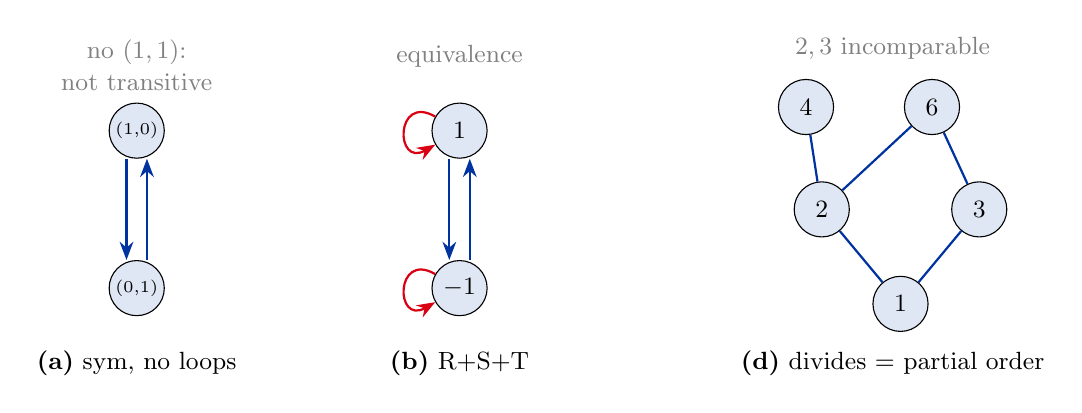
\begin{tikzpicture}[font=\small, >=Stealth,
  vtx/.style={circle,draw,fill=armBlue!12,minimum size=7mm,inner sep=0pt}]
% (a) symmetric-only: 2-cycle (1,0)<->(0,1), no loops, no closing edge
\begin{scope}
  \node[vtx] (p) at (0,1.0) {$\scriptstyle(1,0)$};
  \node[vtx] (q) at (0,-1.0) {$\scriptstyle(0,1)$};
  \draw[armBlue,thick,->] ([xshift=-1.3mm]p.south) -- ([xshift=-1.3mm]q.north);
  \draw[armBlue,thick,->] ([xshift=1.3mm]q.north) -- ([xshift=1.3mm]p.south);
  \node at (0,-1.95) {\textbf{(a)} sym, no loops};
  \node[gray] at (0,2.0) {no $(1,1)$:};
  \node[gray] at (0,1.62) {not transitive};
\end{scope}
% (b) equivalence flavour: loops + mirrored arrows on {1,-1}
\begin{scope}[xshift=4.1cm]
  \node[vtx] (u) at (0,1.0) {$1$};
  \node[vtx] (v) at (0,-1.0) {$-1$};
  \draw[armRed,thick,->] (u) .. controls +(150:0.95) and +(210:0.95) .. (u);
  \draw[armRed,thick,->] (v) .. controls +(150:0.95) and +(210:0.95) .. (v);
  \draw[armBlue,thick,->] ([xshift=-1.3mm]u.south) -- ([xshift=-1.3mm]v.north);
  \draw[armBlue,thick,->] ([xshift=1.3mm]v.north) -- ([xshift=1.3mm]u.south);
  \node at (0,-1.95) {\textbf{(b)} R+S+T};
  \node[gray] at (0,1.95) {equivalence};
\end{scope}
% (d) divisibility partial order on {1,2,3,4,6}
\begin{scope}[xshift=8.7cm, yshift=-0.2cm]
  \node[vtx] (n1) at (1.0,-1.0) {$1$};
  \node[vtx] (n2) at (0.0,0.2) {$2$};
  \node[vtx] (n3) at (2.0,0.2) {$3$};
  \node[vtx] (n4) at (-0.2,1.5) {$4$};
  \node[vtx] (n6) at (1.4,1.5) {$6$};
  \draw[armBlue,thick] (n1)--(n2);
  \draw[armBlue,thick] (n1)--(n3);
  \draw[armBlue,thick] (n2)--(n4);
  \draw[armBlue,thick] (n2)--(n6);
  \draw[armBlue,thick] (n3)--(n6);
  \node at (0.9,-1.75) {\textbf{(d)} divides $=$ partial order};
  \node[gray] at (0.9,2.25) {$2,3$ incomparable};
\end{scope}
\end{tikzpicture}
\end{center}

\textbf{Always check.} A brute-force scan computed all four properties directly from their
definitions on finite samples ($\R$ cases on points including the relevant circle/sign points; (c)
on $\{-6,\dots,6\}\setminus\{0\}$; (d) on $\{1,\dots,12\}$; (e),(f) up to $14$). Every verdict below
matched, including AS failing for (c) on $\Z$ via $2$ and $-2$, and AS holding for (d) on $\N$. \checkmark

\begin{center}
\renewcommand{\arraystretch}{1.25}
\begin{tabular}{@{}clcccccl@{}}
\toprule
 & Relation & R & S & AS & T & Conclusion\\
\midrule
a) & $x^2+y^2=1$ on $\R^2$ & $\times$ & $\checkmark$ & $\times$ & $\times$ & symmetric only\\
b) & $x^2=y^2$ on $\R^2$ & $\checkmark$ & $\checkmark$ & $\times$ & $\checkmark$ & \textbf{equivalence}\\
c) & divisibility on $\Z^2$ & $\checkmark$ & $\times$ & $\times$ & $\checkmark$ & preorder (not antisym.)\\
d) & divisibility on $\N^2$ & $\checkmark$ & $\times$ & $\checkmark$ & $\checkmark$ & \textbf{partial order} (not total)\\
e) & $\gcd(x,y)=1$ on $\N^2$ & $\times$ & $\checkmark$ & $\times$ & $\times$ & symmetric only\\
f) & $\gcd(x,y)=1$ on $\Z^2$ & $\times$ & $\checkmark$ & $\times$ & $\times$ & symmetric only\\
\bottomrule
\end{tabular}
\end{center}

\answer{a) S only; b) equivalence (R,S,T); c) divisibility on $\Z$: R,T but not AS (preorder); d) divisibility on $\N$: partial order (R,AS,T, not total); e),f) S only.}

\begin{methodbox}
\textbf{Transferable technique:} test each property as a picture - reflexive $=$ all loops,
symmetric $=$ all arrows reversible, antisymmetric $=$ no distinct 2-cycle, transitive $=$ shortcuts
present. \emph{One} counterexample kills a property. Two famous packages: R+S+T $=$ equivalence,
R+AS+T $=$ partial order. The same predicate can change class with the ground set: divisibility is a
partial order on $\N$ but only a preorder on $\Z$ (because $n$ and $-n$ divide each other).
\end{methodbox}

% ============================================================================
\section*{Problem 7.2 - Reflexive, symmetric, transitive closures}
% ============================================================================

\begin{problembox}[7.2]
On $A=\{1,2,3,4\}$ let $\rho=\{(1,2),(3,1),(3,2),(2,4)\}$. Find the reflexive closure $r(\rho)$,
the symmetric closure $s(\rho)$, and the transitive closure $t(\rho)$.
\end{problembox}

\begin{ideabox}
A \textbf{closure} is the \emph{smallest} enlargement of $\rho$ that gains a desired property while
adding nothing unnecessary. Each closure has a one-line recipe that says exactly which arrows are
\textquotedbl{}forced\textquotedbl{}:
\[
r(\rho)=\rho\cup\Delta_A\ \ (\text{add every loop}),\qquad
s(\rho)=\rho\cup\rho^{-1}\ \ (\text{add every reverse}),
\]
\[
t(\rho)=\bigcup_{k\ge1}\rho^{\,k}\ \ (\text{add an arrow for every directed path}).
\]
Reading them on the digraph: $r$ stamps a loop on each vertex; $s$ makes every arrow two-way; $t$
asks \textquotedbl{}where can I get to by following arrows?\textquotedbl{} and draws a direct arrow
to every reachable vertex. Closures only \emph{add} edges - the original arrows always stay.
\end{ideabox}

\textbf{Step 1 - Draw $\rho$ and find what each closure must add.}
Reachability in $\rho$: $1\to2\to4$, and $3\to1\to2\to4$ (also $3\to2\to4$).
So the new \emph{transitive} arrows are $1\to4$ (path $1\to2\to4$) and $3\to4$ (path $3\to1\to2\to4$);
note $3\to2$ is already present.

\textbf{Step 2 - Apply the three recipes.}
\begin{align*}
r(\rho)&=\rho\cup\{(1,1),(2,2),(3,3),(4,4)\}\\
&=\{(1,2),(3,1),(3,2),(2,4),\ (1,1),(2,2),(3,3),(4,4)\}.\\[3pt]
s(\rho)&=\rho\cup\rho^{-1}
=\{(1,2),(2,1),(3,1),(1,3),(3,2),(2,3),(2,4),(4,2)\}.\\[3pt]
t(\rho)&=\rho\cup\{(1,4),(3,4)\}
=\{(1,2),(2,4),(3,1),(3,2),\ (1,4),(3,4)\}.
\end{align*}

\textbf{Before / after on the digraph} (original arrows in blue, \textcolor{armRed}{added arrows in red}):

\begin{center}
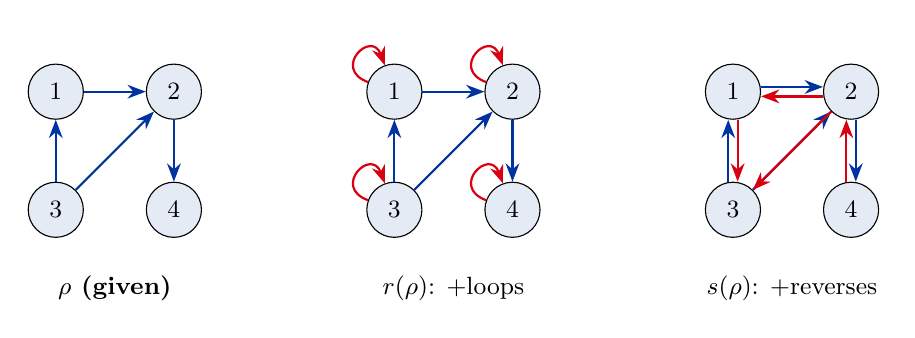
\begin{tikzpicture}[font=\small, >=Stealth, baseline,
  vtx/.style={circle,draw,fill=armBlue!10,minimum size=7mm,inner sep=0pt}]
% --- original rho ---
\begin{scope}
  \node[vtx] (1) at (0,1.5) {$1$};
  \node[vtx] (2) at (1.5,1.5) {$2$};
  \node[vtx] (3) at (0,0) {$3$};
  \node[vtx] (4) at (1.5,0) {$4$};
  \draw[armBlue,thick,->] (1)--(2);
  \draw[armBlue,thick,->] (3)--(1);
  \draw[armBlue,thick,->] (3)--(2);
  \draw[armBlue,thick,->] (2)--(4);
  \node at (0.75,-1.0) {\textbf{$\rho$ (given)}};
\end{scope}
% --- r(rho) ---
\begin{scope}[xshift=4.3cm]
  \node[vtx] (1) at (0,1.5) {$1$};
  \node[vtx] (2) at (1.5,1.5) {$2$};
  \node[vtx] (3) at (0,0) {$3$};
  \node[vtx] (4) at (1.5,0) {$4$};
  \draw[armBlue,thick,->] (1)--(2);
  \draw[armBlue,thick,->] (3)--(1);
  \draw[armBlue,thick,->] (3)--(2);
  \draw[armBlue,thick,->] (2)--(4);
  \foreach \n in {1,2,3,4}
    \draw[armRed,thick,->] (\n) .. controls +(160:0.85) and +(110:0.85) .. (\n);
  \node at (0.75,-1.0) {\textbf{$r(\rho)$}: $+$loops};
\end{scope}
% --- s(rho) ---
\begin{scope}[xshift=8.6cm]
  \node[vtx] (1) at (0,1.5) {$1$};
  \node[vtx] (2) at (1.5,1.5) {$2$};
  \node[vtx] (3) at (0,0) {$3$};
  \node[vtx] (4) at (1.5,0) {$4$};
  \draw[armBlue,thick,->] ([yshift=0.6mm]1.east)--([yshift=0.6mm]2.west);
  \draw[armBlue,thick,->] ([xshift=-0.6mm]3.north)--([xshift=-0.6mm]1.south);
  \draw[armBlue,thick,->] (3)--(2);
  \draw[armBlue,thick,->] ([xshift=0.6mm]2.south)--([xshift=0.6mm]4.north);
  % reverses
  \draw[armRed,thick,->] ([yshift=-0.6mm]2.west)--([yshift=-0.6mm]1.east);
  \draw[armRed,thick,->] ([xshift=0.6mm]1.south)--([xshift=0.6mm]3.north);
  \draw[armRed,thick,->] (2)--(3);
  \draw[armRed,thick,->] ([xshift=-0.6mm]4.north)--([xshift=-0.6mm]2.south);
  \node at (0.75,-1.0) {\textbf{$s(\rho)$}: $+$reverses};
\end{scope}
\end{tikzpicture}
\end{center}

\begin{center}
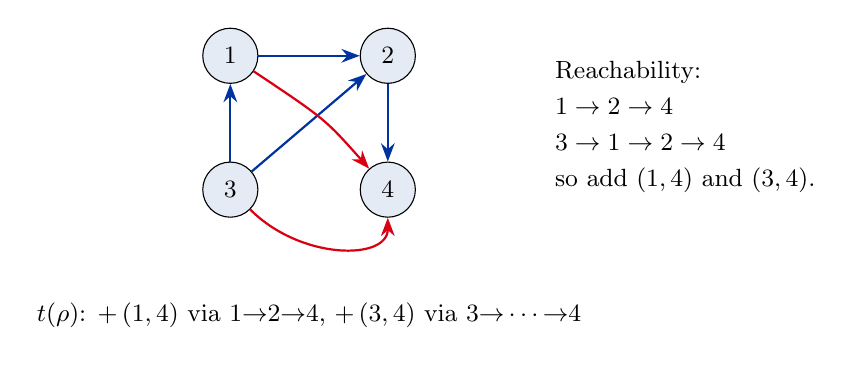
\begin{tikzpicture}[font=\small, >=Stealth, baseline,
  vtx/.style={circle,draw,fill=armBlue!10,minimum size=7mm,inner sep=0pt}]
% --- t(rho) with added arrows ---
\begin{scope}
  \node[vtx] (1) at (0,1.7) {$1$};
  \node[vtx] (2) at (2.0,1.7) {$2$};
  \node[vtx] (3) at (0,0) {$3$};
  \node[vtx] (4) at (2.0,0) {$4$};
  \draw[armBlue,thick,->] (1)--(2);
  \draw[armBlue,thick,->] (3)--(1);
  \draw[armBlue,thick,->] (3)--(2);
  \draw[armBlue,thick,->] (2)--(4);
  % added: 1->4 (path 1-2-4) and 3->4 (path 3-..-4)
  \draw[armRed,thick,->] (1) .. controls (1.2,0.9) .. (4);
  \draw[armRed,thick,->] (3) .. controls (0.9,-0.9) and (2.0,-0.9) .. (4);
  \node at (1.0,-1.6) {\textbf{$t(\rho)$}: $+\,(1,4)$ via $1{\to}2{\to}4$,\ $+\,(3,4)$ via $3{\to}\cdots{\to}4$};
\end{scope}
\node[align=left,anchor=west] at (4.0,0.8)
 {Reachability:\\[2pt]
  $1\to2\to4$\\[2pt]
  $3\to1\to2\to4$\\[2pt]
  so add $(1,4)$ and $(3,4)$.};
\end{tikzpicture}
\end{center}

\textbf{Always check.} The transitive closure was recomputed by Warshall's algorithm on the four
nodes; it returned exactly $\{(1,2),(1,4),(2,4),(3,1),(3,2),(3,4)\}$, matching the by-hand answer.
The reflexive and symmetric closures were verified by directly applying $\rho\cup\Delta_A$ and
$\rho\cup\rho^{-1}$. \checkmark

\answer{$r(\rho)=\rho\cup\{(1,1),(2,2),(3,3),(4,4)\}$;\quad
$s(\rho)=\{(1,2),(2,1),(1,3),(3,1),(2,3),(3,2),(2,4),(4,2)\}$;\quad
$t(\rho)=\{(1,2),(2,4),(3,1),(3,2),(1,4),(3,4)\}$.}

\begin{methodbox}
\textbf{Transferable technique:} closures have fixed recipes - $r=\rho\cup\Delta$,
$s=\rho\cup\rho^{-1}$, $t=\bigcup_k\rho^k$ - and each only \emph{adds} edges. For $t$, the clean way
is reachability: draw an arrow $x\to z$ whenever a directed path goes from $x$ to $z$ (Warshall's
algorithm mechanises exactly this). On a digraph: $r$ stamps every loop, $s$ doubles every arrow,
$t$ shortcuts every path.
\end{methodbox}

\end{document}
